\documentclass[12pt]{article}
\usepackage{amsmath,amssymb,bm,epsf,epsfig,graphicx,hyperref,physics, cleveref, subfig, slashed, stmaryrd, tensor, float}
\captionsetup[subfloat]{labelformat=empty}
\usepackage[backend=bibtex,natbib,style=numeric-comp,sorting=none,maxbibnames=99,doi=false,isbn=false,url=false]{biblatex}
\addbibresource{references.bib}
\input epsf.sty
\topmargin -.5cm \textheight 21cm \oddsidemargin -.125cm
\textwidth 17cm
\setlength{\parskip}{0.7em}

\usepackage[]{todonotes}
\usepackage{tikz}
\usetikzlibrary{arrows.meta, decorations.markings}

\usepackage[weather, alpine]{ifsym}

\def\ie{\begin{equation}\begin{aligned}}
\def\fe{\end{aligned}\end{equation}}
\def\NS{\mathrm{NS}}
\def\R{\mathrm{R}}

\renewcommand{\title}[1]{\vbox{\center\LARGE{#1}}\vspace{5mm}}
\renewcommand{\author}[1]{\vbox{\center#1}\vspace{5mm}}
\newcommand{\address}[1]{\vbox{\center\em#1}}
\newcommand{\email}[1]{\vbox{\center\tt#1}\vspace{5mm}}

\newtheorem{theorem}{Theorem}
\newtheorem{proposition}{Proposition}
\newtheorem{lemma}{Lemma}
\newtheorem{definition}{Definition}

\begin{document}

\unitlength = .8mm

\begin{titlepage}

\begin{center}

\hfill \\
\hfill \\
\vskip 1cm

\title{All-Genus 2D \texorpdfstring{$\mathcal{N}=1$}{N=1} Superconformal Blocks}

\author{Sam Christian, Yuchen Wang, Xi Yin, Yutai Zhang}

\address{Jefferson Physical Laboratory, Harvard University,
Cambridge, MA 02138 USA
}

\email{
    samchristian@fas.harvard.edu, yuchen\_wang@fas.harvard.edu, xiyin@fas.harvard.edu, yutaizhang@fas.harvard.edu}

\end{center}

\abstract{We develop a numerical algorithm for two-dimensional $\mathcal{N}=1$ superconformal blocks at arbitrary genera, in arbitrary plumbing channels, and for arbitrary spin structures. The algorithm utilizes two commuting copies of Virasoro subalgebras of the direct sum of the $\mathcal{N}=1$ superconformal algebra with an auxiliary free fermion, which allows us to reduce the $\mathcal{N}=1$ superconformal blocks to Virasoro conformal blocks.}

\vfill

\end{titlepage}

\eject

\begingroup
\hypersetup{linkcolor=black}

\endgroup

\section{Introduction}

Superconformal blocks are the central objects for computing correlators of superconformal field theories (SCFTs). Given the superconformal block on a spin Riemann surface, together with the conformal data of the SCFT, namely the conformal weights and the structure constants, correlators of a 2-dimensional $\mathcal{N}=1$ SCFT on that spin Riemann surface can be computed through the superconformal block decomposition. 
%These correlators are essential for computing superstring amplitudes and can be used to bootstrap the superconformal data in the modular bootstrap program.

On spin Riemann surfaces of genus $g=0$ or $g=1$, algorithms for numerically computing the superconformal blocks are well developed. Analogously to the Zamolodchikov recursion relation for the sphere 4-point Virasoro conformal block \cite{Zamolodchikov:1984eqp,Zamolodchikov:1987avt}, the sphere 4-point superconformal block on a sphere can be computed using recursion relations in the central charge $c$ or in the intermediate conformal weights $h$. These recursion relations have been worked out for both the case with all-NS external states \cite{Hadasz:2006qb,Hadasz:2007nt,Belavin:2007zz} and that with Ramond external states \cite{Hadasz:2008dt,Suchanek:2010kq}. The $c$-recursion relation can be generalized to arbitrary plumbing channels and arbitrary genus as long as all intermediate states are in the NS sector \cite{Cho:2017oxl,Belavin:2018hfm}. Meanwhile, for the blocks that involve Ramond intermediate states, the $h$-recursion relations can only be generalized to genus 1 \cite{Hadasz:2012im} while the $c$-recursion relation does not exist beyond tree level, due to the fact that the large-$h$ or large-$c$ limit of the Ramond conformal blocks does not exist at higher genus. Algorithms for numerically computing these higher-genus Ramond blocks are absent in the literature.

In this work, we present the first numerical algorithm for these higher-genus Ramond blocks. The algorithm is based on the fact that the $\mathcal{N}=1$ superconformal algebra $\mathsf{SCA}$, direct summed with an auxiliary free fermion algebra $\mathsf{F}$, admits two copies of commuting Virasoro subalgebras \cite{Bershtein:2014yia,Bershtein:2016uov}. These subalgebras were first discovered in the context of the AGT relation \cite{Alday:2009aq,Belavin:2011sw} and have been used in the context of the super-Liouville/double Liouville correspondence \cite{Schomerus:2012se,Hadasz:2013dza}. Using this $\mathsf{Vir}\oplus \mathsf{Vir}$ subalgebra, the superconformal block can be reduced to a sum of products of two Virasoro conformal blocks, which can be computed numerically as a series in the plumbing parameters using the $c$-recursion relation developed in \cite{Cho:2017oxl}.

The rest of this paper is organized as follows. In Section \ref{sec:scblock}, we define the superconformal blocks using the plumbing fixture. In Section \ref{sec:2Vir}, we review the details of the $\mathsf{Vir}\oplus \mathsf{Vir}$ subalgebra and the branching rules of $\mathsf{SCA}\oplus \mathsf{F}$ supermultiplets. In Section \ref{sec:blockdecomp}, we derive the relation between superconformal blocks and Virasoro blocks for blocks without a certain type of obstruction which we call odd Ramond loops. Section \ref{sec:oddloop} extends the construction to blocks with odd Ramond loops using an auxiliary fermion insertion. We present numerical tests for the algorithm in Section \ref{sec:numerics} and discuss applications and future directions in Section \ref{sec:disc}.

\section{The superconformal blocks}

\label{sec:scblock}

An arbitrary punctured Riemann surface can be constructed by gluing 3-punctured Riemann spheres using the plumbing fixture, which takes two punctures with local coordinates $z_1, z_2$ and identifies a pair of annular regions using
\ie 
z_1z_2=q,\quad |q|\leq 1,
\fe
where $q$ is a complex plumbing parameter. A genus-$g$, $n$-punctured Riemann surface can be constructed by plumbing $(3g-3+n)$ pairs of punctures, and its $(3g-3+n)$ complex moduli are given by those $(3g-3+n)$ plumbing parameters. One can then describe a punctured Riemann surface using a trivalent graph $\Gamma$ together with a $q$-parameter for each internal edge. The vertices of $\Gamma$ correspond to the 3-punctured spheres, while the edges connect pairs of plumbed punctures. We call this graph $\Gamma$ a plumbing channel. An example of such a construction, the genus-2 theta channel, is shown in figure \ref{fig:thetachannel}.

\begin{figure}
\begin{center}
        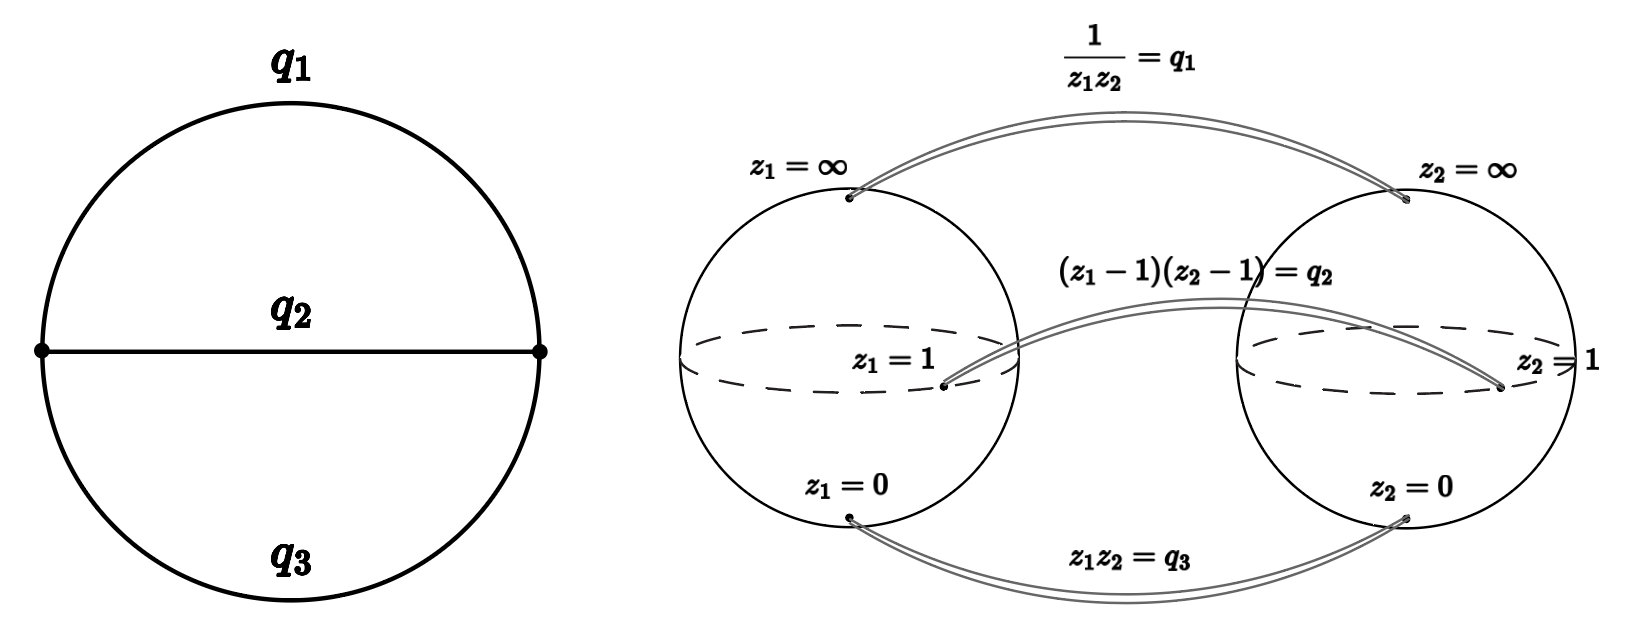
\includegraphics[scale=0.56]{figures/thetachannel.png}
    \end{center}
    \caption{The genus-2 "theta" channel, where the left picture shows the trivalent graph $\Gamma$, and the right picture shows the plumbing performed to construct a genus-2 Riemann surface.}
    \label{fig:thetachannel}
\end{figure}

To specify a spin structure on the Riemann surface, we assign a sign $\eta_e$ for each internal edge $e$ in $\Gamma$, and additionally label each edge of $\Gamma$ by NS or R. In the $\mathcal{N}=1$ SCFT language, $\eta_e$ specifies whether there is a line operator insertion $(-1)^F$ around the tube associated with edge $e$, while the NS/R label specifies the fermionic boundary conditions of the states propagating along the tube. At each vertex, only edges of types (NS, NS, NS) or (NS, R, R) can be connected together. We denote the plumbing graph with the NS/R labels by $\hat{\Gamma}$, and the data of the spin Riemann surface is specified by $(\hat{\Gamma}, \{q_e, \eta_e\})$. The sets of all NS internal edges, R internal edges, (NS, NS, NS) vertices and (NS, R, R) vertices in $\hat{\Gamma}$ are denoted by $E_{\NS}, E_{\R}, V_{\NS}$ and $V_{\R}$, respectively. We also include in $\hat{\Gamma}$ the order of the three half-edges that connect to each vertex, with the first half-edge corresponding to the operator inserted at $z=\infty$, the second corresponding to $z=1$, and the third corresponding to $z=0$. On a (NS, R, R) sphere, we always take the NS half-edge to be in the first slot.

Plumbing two punctures in an SCFT correlator amounts to summing over a complete basis of intermediate states. These states organize into supermultiplets. We denote an NS superconformal primary by $\phi$. A Ramond supermultiplet has 2 ground states $w^\pm$ that are related by $G_0$:
\ie
G_0 w^\pm = i \beta e^{\mp i\pi/4} w^\mp,
\fe
where $\beta$ is defined by $\beta^2 = \frac{c}{24}-h$. We take $w^+$ to be Grassmann even, and hence $w^-$ will be Grassmann odd. A basis of states in a supermultiplet is given by 
\ie
&\mathbf{L}_{-A}\phi \equiv L_{-n_1}\cdots L_{-n_\ell} G_{-r_1}\cdots G_{-r_p} \phi,\\
&\mathbb{L}_{-A} w^\pm \equiv L_{-n_1}\cdots L_{-n_\ell} G_{-r_1}\cdots G_{-r_p} w^\pm,
\fe
in the NS and R sectors, respectively. Here, $n_i\in \mathbb{Z}, r_j\in \mathbb{Z}+\nu$, and $n_1 \geq ... \geq n_\ell>0, r_1>...>r_p>0$, where $\nu=0$ in the R sector and $\nu=\frac{1}{2}$ in the NS sector. We further define the total level of $\mathbf{L}_{-A}, \mathbb{L}_{-A}$ by $|A|\equiv \sum_{i=1}^\ell n_i + \sum_{j=1}^{p} r_j$, and their Grassmann parity by $(-1)^A \equiv (-1)^{p}$.  

After replacing each pair of plumbed punctures by a pair of local operators, the SCFT correlator can be reduced to a product of 3-point functions on the spheres. On an (NS, NS, NS) sphere, all these 3-point functions of descendants can be reduced to either $\langle \phi_1 \phi_2 \phi_3\rangle $ or $\langle \phi_1 (G_{-\frac{1}{2}}\phi_2) \phi_3\rangle $ by superconformal Ward identities. We define the normalized 3-point functions $\rho_a$ by
\ie
\rho_0(\phi_1, \phi_2, \phi_3)=1,\quad \rho_1(\phi_1, G_{-\frac{1}{2}}\phi_2, \phi_3)=1,
\fe
where the operators $\phi_1, \phi_2, \phi_3$ are inserted at $\infty, 1, 0$, respectively. The normalized three-point functions $\rho_a(\mathbf{L}_{-A}\phi_1, \mathbf{L}_{-B}\phi_2,\mathbf{L}_{-C}\phi_3)$ of descendants are defined by reducing them to $\rho_0(\phi_1, \phi_2, \phi_3)$, $\rho_1(\phi_1, G_{-\frac{1}{2}}\phi_2, \phi_3)$ using superconformal Ward identities. On an (NS, R, R) sphere, there are 4 independent 3-point functions, and we define 
\ie
&\rho^{(\eta)}_0(\phi_1, w^+_2, w_3^+) = 1,\quad \rho^{(\eta)}_0(\phi_1, w^-_2, w_3^-) = \eta,\\
&\rho^{(\eta)}_1(\phi_1, w^+_2, w_3^-) = 1,\quad \rho^{(\eta)}_1(\phi_1, w^-_2, w_3^+) = -i\eta,
\fe
for $\eta = \pm$. Again, the operators $\phi_1, w_2^\pm, w_3^\pm$ are inserted at $\infty, 1, 0$, respectively, and the normalized 3-point functions of descendants are defined through superconformal Ward identities. 

On a spin Riemann surface specified by the plumbing data $(\hat{\Gamma}, \{q_e, \eta_e\})$, the superconformal block with internal weights $\{h_e\}_{e\in E_{\NS}}, \{\beta_e\}_{e\in E_\R}$ is defined as
\ie \label{scblock}
\mathbf{F}{}^{\{f, \eta, a\}}_{\hat{\Gamma}}(h_e, \beta_e; q_e, \eta_e) &= \sum_{\{A, \alpha\}}(-1)^{K_{\Gamma}(\epsilon)} \prod_{e\in E_\NS\cup E_\R} q_e^{|A_{e_1}|}\eta_e^{\epsilon_e}\\
&\times \prod_{e\in E_\NS} \mathbf{G}_{h_e}^{A_{e_1}A_{e_2}} \prod_{e\in E_\R} \mathbb{G}_{\beta_e}^{A_{e_1}\alpha_{e_1},A_{e_2}\alpha_{e_2}}\\
&\times \prod_{v \in V_\NS} \rho_{a_v}(\mathbf L_{-A_{v_1}}\phi_{v_1},\mathbf L_{-A_{v_2}}\phi_{v_2},\mathbf L_{-A_{v_3}}\phi_{v_3})\\
&\times\prod_{v\in V_\R}\rho_{f_v}^{(\eta_v)}(\mathbf L_{-A_{v_1}}\phi_{v_1},\mathbb L_{-A_{v_2}}w_{v_2}^{\alpha_{v_2}},\mathbb L_{-A_{v_3}}w_{v_3}^{\alpha_{v_3}}),
\fe
where $f_v, \eta_v$ label the 3-point functions on the (NS, R, R) spheres, and $a_v$ labels those on the (NS, NS, NS) spheres. The two half-edges an edge $e$ contains are labeled $e_1, e_2$, and the three half-edges connected to a vertex $v$ are labeled $v_1, v_2, v_3$ according to their aforementioned order \footnote{The order of the two half-edges in an edge does not matter, since the Grassmann sign of exchanging $\Phi_A, \Phi_B$ is cancelled by the relative sign between $\mathbf{G}^{AB}$ and $\mathbf{G}^{BA}$.}. The sum is over all displayed descendant labels $A$ and ground state labels $\alpha$ on each half-edge, subject to the conditions
\ie \label{selection}
&|A_{e_1}| = |A_{e_2}|,\quad e\in E_{\NS}\cup E_\R\\
&(-1)^{A_{v_1}+A_{v_2}+A_{v_3}}=(-1)^{a_v},\quad v\in V_\NS,\\
&(-1)^{A_{v_1}+A_{v_2}+A_{v_3}+\alpha_{v_2}+\alpha_{v_3}}=(-1)^{f_v},\quad v\in V_\R.
\fe
We define $\epsilon_{v_i}$ to be the total Grassmann parity of the descendant $\Phi_{v_i}$, which stands for $\mathbf{L}_{-A_{v,i}}\phi_{v_i}$ in the NS sector or $\mathbb{L}_{-A_{v_i}}w_{v_i}^{\alpha_{v_i}}$ in the R sector. The sign $(-1)^{K_\Gamma(\epsilon)}$ is the Grassmann sign that arises from moving the operator order from the pairwise insertion order to the displayed order in the 3-point functions \footnote{More explicitly, this is the Grassmann sign that arises from moving the operators from order $\prod_{e\in E_\NS\cup E_\R}\Phi_{e_1}\Phi_{e_2}$ to order $\prod_{v\in V_\NS}\Phi_{v_1}\Phi_{v_2}\Phi_{v_3}\prod_{v\in V_\R}\Phi_{v_1}\Phi_{v_2}\Phi_{v_3}$. It can be defined as $(-1)^{K_\Gamma(\epsilon)}=\sum_{(v_i, w_j)}\epsilon_{v_i}\epsilon_{w_j}$, where the sum is over pairs $(v_i, w_j)$ such that $v_i$ precedes $w_j$ in the pairwise insertion but the opposite in the order of the 3-point functions.}. $\mathbf{G}, \mathbb{G}$ are inverse Gram matrices in the NS and R sectors, which are defined as the inverse of
\ie
(\mathbf{G}_h)_{AB}&=\langle\langle \mathbf{L}_{-A}\phi_h|\mathbf{L}_{-B}\phi_h\rangle,\\
(\mathbb{G}_\beta)_{A\alpha, B\alpha'}&=\langle\langle \mathbb{L}_{-A}w_\beta^\alpha|\mathbb{L}_{-B}w_\beta^{\alpha'}\rangle,
\fe
where the double left bracket stands for BPZ conjugation. $h, \beta$ label the conformal weight and $G_0$ eigenvalues of the primaries, which are normalized such that $\langle\langle \phi_h|\phi_h\rangle =1$, $\langle\langle w_\beta^+|w_\beta^{+} \rangle=1$. In the rest of this paper, we will omit the labels $(h_e, \beta_e;q_e, \eta_e)$ when writing the superconformal block. 

% For simplicity, we will focus on the genus-2 theta channel in the rest of this Letter, where we sew together $z_1=z_2=0$, $z_1=z_2=1$ and $z_1=z_2=\infty$ on two Riemann spheres with complex coordinates $z_1, z_2$. The two edges that connect $z_1=z_2=0,1$ are R, while the edge that connects $z_1=z_2=\infty$ is NS. Nevertheless, the algorithm we present here can be easily generalized to arbitrary plumbing channels and arbitrary spin structures, and we leave the details to the appendix. \textbf{[Figure: Theta channel]}

% In the genus-2 theta channel, the superconformal block with internal weights $h_{1}, \beta_2, \beta_3$ is defined as
% \ie \label{scblock}
% &\mathbf{F}^{(\eta, \eta')}_f(h_1, \beta_2, \beta_3)=\\
% &\sum_{\substack{|A|=|A'|, |B|=|B'|, |C|=|C'|\\ (-1)^{A+B+C+|\alpha|+|\gamma|}=(-1)^f\\(-1)^{A'+B'+C'+|\alpha'|+|\gamma'|}=(-1)^f}} q_1^{|A|} \eta_1^{\epsilon_1} q_2^{|B|} \eta_2^{\epsilon_2} q_3^{|C|} \eta_3^{\epsilon_3} \\
% &\quad\quad \times (-1)^{\epsilon_1\epsilon_2+\epsilon_1\epsilon_3+\epsilon_2\epsilon_3}\mathbf{G}^{AA'}_{h_1} \mathbb{G}^{B\alpha, B'\alpha'}_{\beta_2} \mathbb{G}^{C\gamma, C'\gamma'}_{\beta_3}\\
% &\quad\quad \times \rho_f^{(\eta)}(\mathbf{L}_{-A}\phi_1, \mathbb{L}_{-B}w^\alpha_2, \mathbb{L}_{-C}w^\gamma_3)\\
% &\quad\quad \times \rho_f^{(\eta')}(\mathbf{L}_{-A'}\phi_1, \mathbb{L}_{-B'}w^{\alpha'}_2, \mathbb{L}_{-C'}w^{\gamma'}_3),
% \fe
% where the sum is over all displayed descendant labels and ground state labels. This will be true throughout this letter. $\eta, \eta'$, and $f$ label the three-point functions on the two (NS, R, R) spheres, and the two $f$ labels are forced to be the same by the Gram matrices. $\epsilon_{1,2,3}$ are defined to be the total Grassmann parity of $\mathbf{L}_{-A}\phi_1, \mathbb{L}_{-B}w_2^\alpha$ and $\mathbb{L}_{-C}w_3^\gamma$, respectively \footnote{The sign on the second line is the Grassmann sign that arises when reordering the operators from the pairwise insertion order $\mathbf{L}_{-A}\phi_1\mathbf{L}_{-A'}\phi_1\mathbb{L}_{-B}w^\alpha_2\mathbb{L}_{-B'}w^{\alpha'}_2\mathbb{L}_{-C}w^\gamma_3\mathbb{L}_{-C'}w^{\gamma'}_3$ to the displayed order in the three-point functions.}. $\mathbf{G}, \mathbb{G}$ are inverse Gram matrices in the NS and R sectors, which are defined as the inverse of
% \ie
% (\mathbf{G}_h)_{AB}&=\langle\langle \mathbf{L}_{-A}\phi_h|\mathbf{L}_{-B}\phi_h\rangle\\
% (\mathbb{G}_\beta)_{A\alpha, B\alpha'}&=\langle\langle \mathbb{L}_{-A}w_\beta^\alpha|\mathbb{L}_{-B}w_\beta^{\alpha'}\rangle
% \fe
% where the double left bracket stands for BPZ conjugation. $h, \beta$ label the conformal weight and $G_0$ eigenvalues of the primaries, which are normalized such that $\langle\langle \phi_h|\phi_h\rangle =1$, $\langle\langle w_\beta^+|w_\beta^{+} \rangle=1$.

% Given a parity $a_v=0,1$ for each (NS, NS, NS) vertex and $f_v=0,1, \eta_v=\pm$ for each (NS, R, R) vertex in $\hat{\Gamma}$, The superconformal block on a spin Riemann surface $(\hat{\Gamma}, \{q_e, \eta_e\})$ is defined as
% \begin{widetext}
% \ie
% \mathbf{F}_{\hat{\Gamma}}^{(a_v, f_v, \eta_v)}(h_e, p_e &; q_e, \eta_e) = \sum_{\{A, \alpha\}} \mathrm{sgn}(\hat{\Gamma}) \prod_{e\in E_{\NS}(\hat{\Gamma})}q_e^{|A_{e,1}|}\eta_e^{A_{e,1}+p_{e,1}}\mathbf{G}^{A_{e,1}A_{e,2}}_{h_e} \prod_{e \in E_{\R}(\hat{\Gamma})} q_{e}^{|A_{e,1}|}\eta_{e}^{A_{e,1}+|\alpha_{e,1}|}\mathbb{G}^{A_{e,1}\alpha_{e}, A_{e,2}\alpha_{e,2}}_{\beta_{e}}\\
% &\times \prod_{v\in V_{\NS}} \rho_{a_v}(\mathbf{L}_{-A_{v,1}}\phi_{h_{v,1}}, \mathbf{L}_{-A_{v,2}}\phi_{h_{v,2}}, \mathbf{L}_{-A_{v,3}}\phi_{h_{v,3}}) \times \prod_{v\in V_{\R}} \rho_{f_v}^{(\eta_v)}(\mathbf{L}_{-A_{v,1}}\phi_{h_{v,1}}, \mathbb{L}_{-A_{v,2}}w_{\beta_{v,2}}^{\alpha_{v,2}}, \mathbb{L}_{-A_{v,3}}w_{\beta_{v,3}}^{\alpha_{v,3}})
% \fe
% \end{widetext}
%   For each edge $v$, $A_{e,1}, A_{e,2}$ are the two descendant labels on the two half-edges. Similarly for each vertex $v$, $A_{v,1}, A_{v,2}, A_{v,3}$ are the labels of the three half-edges it connects. The sign $\mathrm{sgn}(\hat{\Gamma})$ is the Grassmann sign that arises from moving the operator order from 
% \[
% \prod_{e\in E_{\NS}(\hat{\Gamma})}\mathbf{L}_{-A_{e,1}}\phi_{h_e}\mathbf{L}_{-A_{e,2}}\phi_{h_e}\prod_{e\in E_{\R}(\hat{\Gamma})}\mathbb{L}_{-A_{e,1}}w_{\beta_e}^{\alpha_{e,1}}\mathbb{L}_{-A_{e,2}}w_{\beta_e}^{\alpha_{e,2}}\]
% to the displayed order
% \[\begin{aligned}
% &\prod_{v\in V_{\NS}}\mathbf{L}_{-A_{v,1}}\phi_{h_{v,1}}\mathbf{L}_{-A_{v,2}}\phi_{h_{v,2}}\mathbf{L}_{-A_{v,3}}\phi_{h_{v,3}}\\
% &\quad \quad \times \prod_{v\in V_{\R}} \mathbf{L}_{-A_{v,1}}\phi_{h_{v,1}}\mathbb{L}_{-A_{v,2}}w_{\beta_{v,2}}^{\alpha_{v,2}}\mathbb{L}_{-A_{v,3}}w_{\beta_{v,3}}^{\alpha_{v,3}}.
% \end{aligned}\]

\section{The double Virasoro subalgebra}

\label{sec:2Vir}

The key fact we utilize is that, the enlarged algebra $\mathsf{SCA}_\nu \oplus \mathsf{F}_{\nu}$ constructed from direct summing the $\mathcal{N}=1$ superconformal algebra $\mathsf{SCA}_\nu$ with shift $\nu\in \left\{0,\frac{1}{2}\right\}$ with an auxiliary free fermion algebra $\mathsf{F}_\nu$ with the same shift $\nu$
\ie
\{\psi_r, \psi_s\} &= \delta_{r+s,0},\quad \{\psi_r, G_s\}=[\psi_r, L_n] = 0,
\fe
admits two commuting Virasoro subalgebras \cite{Hadasz:2013dza,Bershtein:2014yia,Bershtein:2016uov}. 

The generators of the two commuting Virasoro algebras can be written down explicitly as the following. We introduce the following operators
\ie
L_n^{\mathrm{F}} &= \frac{1}{2} \sum_{r\in \mathbb{Z}+\nu} r:\psi_{n-r}\psi_r: + \frac{1-2\nu}{16}\delta_{n,0},\quad U_n = \sum_{r\in \mathbb{Z}+\nu} \psi_{n-r} G_r,
\fe
and the Virasoro generators are given by
\ie
& L_n^{(1)}=\frac{b^{-1} L_n-\left(b^{-1}+2 b\right) L_n^{\mathrm{F}}+U_n}{b^{-1}-b}, \quad L_n^{(2)}=\frac{b L_n-\left(b+2 b^{-1}\right) L_n^{\mathrm{F}}+U_n}{b-b^{-1}},
\fe
where $b$ is defined by the $\mathsf{SCA}$ central charge $c= \frac{3}{2}+3\left(b+b^{-1}\right)^2$, and we have assumed that $b\neq 0,1$. These generators $L_n^{(1,2)}$ satisfy $L_n^{(1)}+L_n^{(2)}=L_n+L_n^{\mathrm{F}}$, and the two central charges of the two Virasoro algebras are given by
\ie
c^{(1)}=1+\frac{3 Q^2}{1-b^2}, \quad c^{(2)}=1+\frac{3 Q^2}{1-b^{-2}},
\fe
where the Liouville background charge $Q$ is defined such that $Q=b+b^{-1}$.

Let $\mathcal{M}_{\NS}(h), \mathcal{M}_{\R}(\beta)$ denote the tensor products of the auxiliary fermion Fock space with the corresponding SCFT Verma module. We denote the two R-sector ground states for the free fermion by $u^\mathsf{a}$ with $\mathsf{a}=0,1$, which satisfy
\ie
\psi_0 u^{\mathsf{a}} = \frac{1}{\sqrt{2}} u^{1-\mathsf{a}}.
\fe
The highest weight states in $\mathcal{M}_{\NS}(h), \mathcal{M}_{\R}(\beta)$ are respectively $\mathbf{1}\otimes \phi$ and $u^{\mathsf{a}}\otimes w^\alpha$. For Liouville momentum $P\notin \frac{1}{2}(b\mathbb{Z}+b^{-1}\mathbb{Z})$, these representations have branching rules \cite{Bershtein:2014yia,Bershtein:2016uov}
\ie
\mathcal{M}_{\NS}(h)&\cong\bigoplus_{n\in\frac12\mathbb Z} V_{c^{(1)}}(h_n^{(1)})\otimes V_{c^{(2)}}(h_n^{(2)}),\\
\mathcal{M}_{\R}(\beta)&\cong\bigoplus_{\alpha=0,1}\ \bigoplus_{n\in\frac12\mathbb Z+\frac14} V_{c^{(1)}}(h_n^{(1)})\otimes V_{c^{(2)}}(h_n^{(2)}),
\fe
where $P$ is defined using $P^2=\frac{1}{4}Q^2-2h$ in the NS sector and $P^2=2\beta^2$ in the R sector. Here, $V_c(h)$ is the Virasoro Verma module with highest weight $h$ and central charge $c$. The highest-weight vector in $V_{c^{(1)}}(h_n^{(1)})\otimes V_{c^{(2)}}(h_n^{(2)})$ are denoted by $v_n$ and $v_n^\alpha$ in NS and R sectors, respectively. Their conformal weights are
\ie
h_n^{(1)}=\frac{Q^2/4-(P+2nb)^2}{2(1-b^2)},\quad h_n^{(2)}=\frac{Q^2/4-(P+2nb^{-1})^2}{2(1-b^{-2})}.
\fe
The NS $\mathsf{Vir}\oplus \mathsf{Vir}$ primary $v_n$ has Grassmann parity $2n\bmod2$ and level $2n^2$ relative to $\mathbf{1}\otimes \phi$, and the R primary $v^\alpha_n$ has Grassmann parity $\alpha=0,1$ and level $2n^2-\frac18$ relative to $u^{0}\otimes w^0$. These $\mathsf{Vir\oplus Vir}$ primaries can be realized by a free field representation, which we review in appendix \ref{app:freefield}.

\section{Reduction of superconformal blocks}

\label{sec:blockdecomp}

To reduce the superconformal block \eqref{scblock} to Virasoro conformal blocks, we first consider an enlarged $\mathsf{SCA}\oplus \mathsf{F}$ block $\widehat{\mathbf{F}}^{\{f,\eta,a\}}_{\hat{\Gamma}}$, defined as
\ie 
\widehat{\mathbf{F}}^{\{f,\eta,a\}}_{\hat{\Gamma}} &= \sum_{\{A,\alpha,\mathsf{A},\mathsf{a}\}} (-1)^{K_\Gamma(\epsilon+\epsilon')} \prod_{e\in E_\NS\cup E_\R} q_e^{|A_{e_1}|+|\mathsf{A}_{e_1}|}\eta_e^{\epsilon_e+\epsilon_e'}(-1)^{\epsilon_e'} \prod_{e\in E_\NS} \mathbf{G}_{h_e}^{A_{e_1}A_{e_2}} \prod_{e\in E_\R} \mathbb{G}_{\beta_e}^{A_{e_1}\alpha_{e_1},A_{e_2}\alpha_{e_2}}\\
&\times \prod_{v \in V_\NS} \hat{\rho}_{a_v}(\Psi_{-\mathsf{A}_{v_1}}\mathbf{1}\otimes \mathbf L_{-A_{v_1}}\phi_{v_1},\Psi_{-\mathsf{A}_{v_2}}\mathbf{1}\otimes \mathbf L_{-A_{v_2}}\phi_{v_2},\Psi_{-\mathsf{A}_{v_3}}\mathbf{1}\otimes \mathbf L_{-A_{v_3}}\phi_{v_3})\\
&\times\prod_{v\in V_\R}\hat{\rho}_{f_v}^{(\eta_v)}(\Psi_{-\mathsf{A}_{v_1}}\mathbf{1}\otimes \mathbf L_{-A_{v_1}}\phi_{v_1},\Psi_{-\mathsf{A}_{v_2}} u^{\mathsf{a_{v_2}}}\otimes\mathbb L_{-A_{v_2}}w_{v_2}^{\alpha_{v_2}},\Psi_{-\mathsf{A}_{v_3}} u^{\mathsf{a_{v_3}}}\otimes\mathbb L_{-A_{v_3}}w_{v_3}^{\alpha_{v_3}})
\fe
where $\Psi_{-\mathsf{A}}$ denotes a chain of fermion creation operators $\psi_{-r}$ with $r>0$, and $|\mathsf{A}|$ denotes its total level. The sum is over all displayed descendant and ground state labels, subject to
\ie \label{Fselection}
&\mathsf{A}_{e_1} = \mathsf{A}_{e_2},\quad e\in E_{\NS}\cup E_\R\\
&\mathsf{a}_{e_1} = \mathsf{a}_{e_2},\quad e\in E_\R\\
&(-1)^{\mathsf{A}_{v_1}+\mathsf{A}_{v_2}+\mathsf{A}_{v_3}} = 1,\quad v\in V_{\NS}\\
&(-1)^{\mathsf{A}_{v_1}+\mathsf{A}_{v_2}+\mathsf{A}_{v_3}+\mathsf{a}_{v_2}+\mathsf{a}_{v_3}} = 1,\quad v\in V_{\R},
\fe
in addition to \eqref{selection}. $\epsilon$ and $\epsilon'$ denote the Grassmann parity of the $\mathsf{SCA}$ and the fermion part of the corresponding descendant, respectively. The enlarged 3-point functions $\hat{\rho}_a, \hat{\rho}_f^{(\eta)}$ are defined using the product of the fermion 3-point function and the normalized 3-point functions as
\ie 
 &\hat\rho_a(\Psi_{-\mathsf A}\mathbf1\otimes\mathbf L_{-A}\phi_1,
 \Psi_{-\mathsf B}\mathbf1\otimes\mathbf L_{-B}\phi_2,
 \Psi_{-\mathsf C}\mathbf1\otimes\mathbf L_{-C}\phi_3)\\
 &\qquad=(-1)^{\epsilon_2 \epsilon_3'}
 \rho_{\mathsf{F}}(\Psi_{-\mathsf A}\mathbf1,\Psi_{-\mathsf B}\mathbf1,
                                      \Psi_{-\mathsf C}\mathbf1)
 \rho_a(\mathbf L_{-A}\phi_1,\mathbf L_{-B}\phi_2,\mathbf L_{-C}\phi_3),\\
 &\hat\rho_f^{(\eta)}(\Psi_{-\mathsf A}\mathbf1\otimes\mathbf L_{-A}\phi_1,
 \Psi_{-\mathsf B}u^{\mathsf b}\otimes\mathbb L_{-B}w_2^\alpha,
 \Psi_{-\mathsf C}u^{\mathsf c}\otimes\mathbb L_{-C}w_3^\gamma)\\
 &\qquad=(-1)^{\epsilon_2 \epsilon_3'}
 \rho_{\mathsf{F}}(\Psi_{-\mathsf A}\mathbf1,\Psi_{-\mathsf B}u^{\mathsf b},
                                      \Psi_{-\mathsf C}u^{\mathsf c})
 \rho_f^{(\eta)}(\mathbf L_{-A}\phi_1,\mathbb L_{-B}w_2^\alpha,
                                      \mathbb L_{-C}w_3^\gamma),
\fe
where the fermion 3-point function is normalized by $\rho_{\mathsf{F}}(\mathbf{1,1,1})=1$, $\rho_{\mathsf{F}}(\mathbf{1},u^0,u^0)=1$ and $\rho_{\mathsf{F}}(\mathbf{1},u^1,u^1)=i$.

This enlarged block $\widehat{\mathbf{F}}^{\{f,\eta,a\}}_{\hat{\Gamma}}$ can be computed in two different ways. One can take the basis $\Psi_{-\mathsf{A}}\mathbf{1}\otimes \mathbf{L}_{-A}\phi$ for states in $\mathcal{M}_\NS(h)$ and $\Psi_{-\mathsf{A}}u^{\mathsf{a}}\otimes \mathbb{L}_{-A}w^\alpha$ for $\mathcal{M}_{\R}(\beta)$. This allows us to express the enlarged block in terms of the superconformal block \eqref{scblock} and the free fermion block. Namely,
\ie \label{FconvF}
\widehat{\mathbf{F}}_{\hat{\Gamma}}^{\{f,\eta,a\}} = \mathbf{F}_{\hat{\Gamma}}^{\{f,\eta,a\}} \star \mathbf{F}^{\mathsf{F}}_{\hat{\Gamma}},
\fe
where we view the blocks as formal series in $q_e, \eta_e$, and the convolution $\star$ acts on monomials as
\ie \label{conv}
&\left(\prod_e q_e^{r_e}\eta_e^{\epsilon_e}\right)\star\left(\prod_e q_e^{s_e}\eta_e^{\epsilon'_e}\right) = (-1)^{K(\epsilon+\epsilon')-K(\epsilon)-K(\epsilon')+\sum_v\epsilon_{v,2}\epsilon'_{v,3}}
 \prod_e q_e^{r_e+s_e}\eta_e^{\epsilon_e+\epsilon'_e},
\fe
while the free fermion block $\mathbf{F}_{\mathsf{F}}$ is defined as
\ie
\mathbf{F}^{\mathsf{F}}_{\hat{\Gamma}} &= \sum_{\{\mathsf{A,a}\}} (-1)^{K_\Gamma(\epsilon')} \prod_{e\in E_\NS\cup E_\R} q_e^{|\mathsf{A}_{e_1}|}(-\eta_e)^{\epsilon_e'}\\
&\times \prod_{v\in V_\NS} \rho_{\mathsf{F}}(\Psi_{-\mathsf{A}_{v_1}}\mathbf{1},\Psi_{-\mathsf{A}_{v_2}}\mathbf{1},\Psi_{-\mathsf{A}_{v_3}}\mathbf{1})\\
&\times \prod_{v\in V_\R} \rho_{\mathsf{F}}(\Psi_{-\mathsf{A}_{v_1}}\mathbf{1},\Psi_{-\mathsf{A}_{v_2}}u^{\mathsf{a}_{v_2}},\Psi_{-\mathsf{A}_{v_3}}u^{\mathsf{a}_{v_3}}).
\fe

As is, the enlarged block $\hat{\mathbf{F}}^{(\eta, \eta')}_f$ vanishes whenever the labels $f_v,\eta_v$ in $\rho_f^{(\eta)}$ around a closed Ramond loop $C\subset \hat{\Gamma}$ have product
\ie
(-1)^{\sum_{v\in C} f_v} \prod_{v\in C}\eta_v = -1.
\fe
We call such a loop an odd Ramond loop, and the algorithm for computing superconformal blocks with odd Ramond loops will be presented in Section \ref{sec:oddloop}. In the rest of this section, we assume that there are no such odd Ramond loops.

The enlarged block can also be computed using the basis $L_{-A}^{(1)}L_{-B}^{(2)}v_n$ for $\mathcal{M}_{\NS}(h)$ and $L_{-A}^{(1)}L_{-B}^{(2)}v_n^\alpha$ for $\mathcal{M}_{\R}(\beta)$. This leads to the following decomposition of $\widehat{\mathbf{F}}_{\hat{\Gamma}}^{\{f, \eta, a\}}$:
\ie
\widehat{\mathbf{F}}_{\hat{\Gamma}}^{\{f, \eta, a\}} &= \sum_{\{n,\alpha\}} (-1)^{K(\epsilon)} \prod_{e\in E_\NS} q_e^{2n_e^2}\eta_e^{2n_e} \prod_{e\in E_\R} q_e^{2n_e^2-\frac{1}{8}}\eta_e^{\alpha_e}\\
&\times \prod_{i=1}^2 F_{\Gamma}(h_{e,n_e}^{(i)}, c^{(i)}) \prod_{v\in V_\NS} \mathbf{B}_{a_v}(n_{v_1},n_{v_2},n_{v_3})\\
&\times \prod_{v\in V_\R} \mathbb{B}_{f_v}^{(\eta_v)}(n_{v_1},n_{v_2},n_{v_3},\alpha_{v_2},\alpha_{v_3}),\\
\fe
where the labels $n$ take values in $n\in \frac{1}{2}\mathbb{Z}$ for NS half-edges, and $n\in \frac{1}{2}\mathbb{Z}+\frac{1}{4}$ for R half-edges. $F(h_e; c)$ denotes the Virasoro conformal block in the same channel $\Gamma$ with intermediate weights $h_{e}$ and central charge $c$. $\epsilon$ here denotes the Grassmann parity of the $\mathsf{Vir}\oplus \mathsf{Vir}$ primary $v_n$ or $v_n^\alpha$. $\mathbf{B}_a, \mathbb{B}^{(\eta)}_f$ are the branching coefficients, defined as
\ie \label{branch}
&\mathbf{B}_a(n_1, n_2, n_3) = \frac{\hat{\rho}_a(v_{1,n_1}, v_{2,n_2}, v_{3,n_3})}{\|v_{1,n_1}\|\|v_{2,n_2}\|\|v_{3,n_3}\|},\\
&\mathbb{B}^{(\eta)}_f(n_1, n_2, n_3,\alpha_2, \alpha_3) = \frac{\hat{\rho}_f^{(\eta)}(v_{1,n_1}, v_{2,n_2}^{\alpha_2}, v_{3,n_3}^{\alpha_3})}{\|v_{1,n_1}\|\|v_{2,n_2}^{\alpha_2}\|\|v_{3,n_3}^{\alpha_3}\|}.
\fe

The (NS, NS, NS) branching coefficients have been worked out in \cite{Hadasz:2013dza}, while the (NS, R, R) coefficients have never been computed analytically in the literature. We now present a recursive algorithm for determining both numerically. It can be proved that, for $n> 0$, $L_1 v_n, L_{1}v_n^\alpha$ both only contain level-$(4n-3)$ states in the $\mathsf{Vir\oplus Vir}$ module generated by $v_{n-1}, v_{n-1}^\alpha$, while $L_{-1}v_n, L_{-1}v_n^\alpha$ only contain level-1 states in the $v_n, v_n^\alpha$ module as well as level-$(4n-1)$ states in the $v_{n-1}, v_{n-1}^\alpha$ module. Namely, there exist coefficients $\mathbf{V}_n^{(1,2)}, \mathbf{V}_{\pm 1, n}^{AB}, \mathbb{V}_n^{(1,2)}, \mathbb{V}_{\pm 1, n}^{AB}$ such that
\ie \label{Vcoeffs}
L_1 v_n^\alpha &= \sum_{|A|+|B|=4n-3} \mathbb{V}_{1,n,\alpha}^{AB} L_{-A}^{(1)}L_{-B}^{(2)} v_{n-1}^\alpha,\\
L_{-1} v_n^\alpha &= \mathbb{V}_{n,\alpha}^{(1)} L_{-1}^{(1)}v_n^\alpha + \mathbb{V}_{n,\alpha}^{(2)} L_{-1}^{(2)}v_n^\alpha + \sum_{|A|+|B|=4n-1} \mathbb{V}_{-1,n,\alpha}^{AB} L_{-A}^{(1)}L_{-B}^{(2)} v_{n-1}^\alpha,\\
L_1 v_n &= \sum_{|A|+|B|=4n-3} \mathbf{V}_{1,n}^{AB} L_{-A}^{(1)}L_{-B}^{(2)} v_{n-1},\\
L_{-1} v_n &= \mathbf{V}_{n}^{(1)} L_{-1}^{(1)}v_n + \mathbf{V}_{n}^{(2)} L_{-1}^{(2)}v_n  + \sum_{|A|+|B|=4n-1} \mathbf{V}_{-1,n}^{AB} L_{-A}^{(1)}L_{-B}^{(2)} v_{n-1}.
\fe
These coefficients $\mathbf{V}_n^{(1,2)}, \mathbf{V}_{\pm 1, n}^{AB}, \mathbb{V}_n^{(1,2)}, \mathbb{V}_{\pm 1, n}^{AB}$ can be determined directly by applying the free-field realization of $L_{\pm 1}$ on \eqref{vNS}, \eqref{vR}. A similar relation exists for $n< 0$, where $L_{\pm 1}v_n, L_{\pm 1}v_n^\alpha$ include states in the $v_{n+1}, v_{n+1}^\alpha$ module instead of $v_{n-1}, v_{n-1}^\alpha$.

After determining the coefficients $\mathbb{V}$ and $\mathbf{V}$, one can use the $L_1$ conformal Ward identities
\ie
\hat{\rho}_f^{(\eta)}(L_1v_{1,n_1},v_{2,n_2}^{\alpha_2},v_{3,n_3}^{\alpha_3})&= \hat{\rho}_f^{(\eta)}(v_{1,n_1},L_{-1}v_{2,n_2}^{\alpha_2},v_{3,n_3}^{\alpha_3})+\hat{\rho}_f^{(\eta)}(v_{1,n_1},v_{2,n_2}^{\alpha_2},L_{-1}v_{3,n_3}^{\alpha_3}),\\
\hat{\rho}_f^{(\eta)}(v_{1,n_1},L_1v_{2,n_2}^{\alpha_2},v_{3,n_3}^{\alpha_3})&= \hat{\rho}_f^{(\eta)}(L_{-1}v_{1,n_1},v_{2,n_2}^{\alpha_2},v_{3,n_3}^{\alpha_3})-\hat{\rho}_f^{(\eta)}(v_{1,n_1},L_{-1}v_{2,n_2}^{\alpha_2},v_{3,n_3}^{\alpha_3})\\
&\quad-2\hat{\rho}_f^{(\eta)}(v_{1,n_1},L_0v_{2,n_2}^{\alpha_2},v_{3,n_3}^{\alpha_3})-\hat{\rho}_f^{(\eta)}(v_{1,n_1},v_{2,n_2}^{\alpha_2},L_1v_{3,n_3}^{\alpha_3}),
\fe
which become recursion relations for the branching coefficients $\mathbb{B}(n_1, n_2, n_3)$. Given the boundary values $\mathbb{B}(n_1, n_2, n_3)$ with $-\frac{3}{4}\leq n_i \leq \frac{3}{4}$, which can be computed analytically using the free field realization, one can solve for $\mathbb{B}(n_1, n_2, n_3)$ recursively. 

Once one knows the branching coefficients, one can use the $c$-recursion relation to compute the Virasoro conformal blocks \cite{Cho:2017oxl}, which computes $\widehat{\mathbf{F}}_{\hat{\Gamma}}^{\{f, \eta, a\}}$ as a $q$-series. The free fermion block $\mathbf{F}^{\mathsf{F}}_{\hat{\Gamma}}$ can be computed from its definition efficiently due to the small size of the space of fermion descendants. The superconformal block $\mathbf{F}_{\hat{\Gamma}}^{\{f, \eta, a\}}$, as a series in $\{\eta_e, q_e\}$, can be extracted coefficient-by-coefficient from \eqref{FconvF}.

\section{Blocks with odd Ramond loops}

\label{sec:oddloop}

\begin{figure}
\begin{center}
        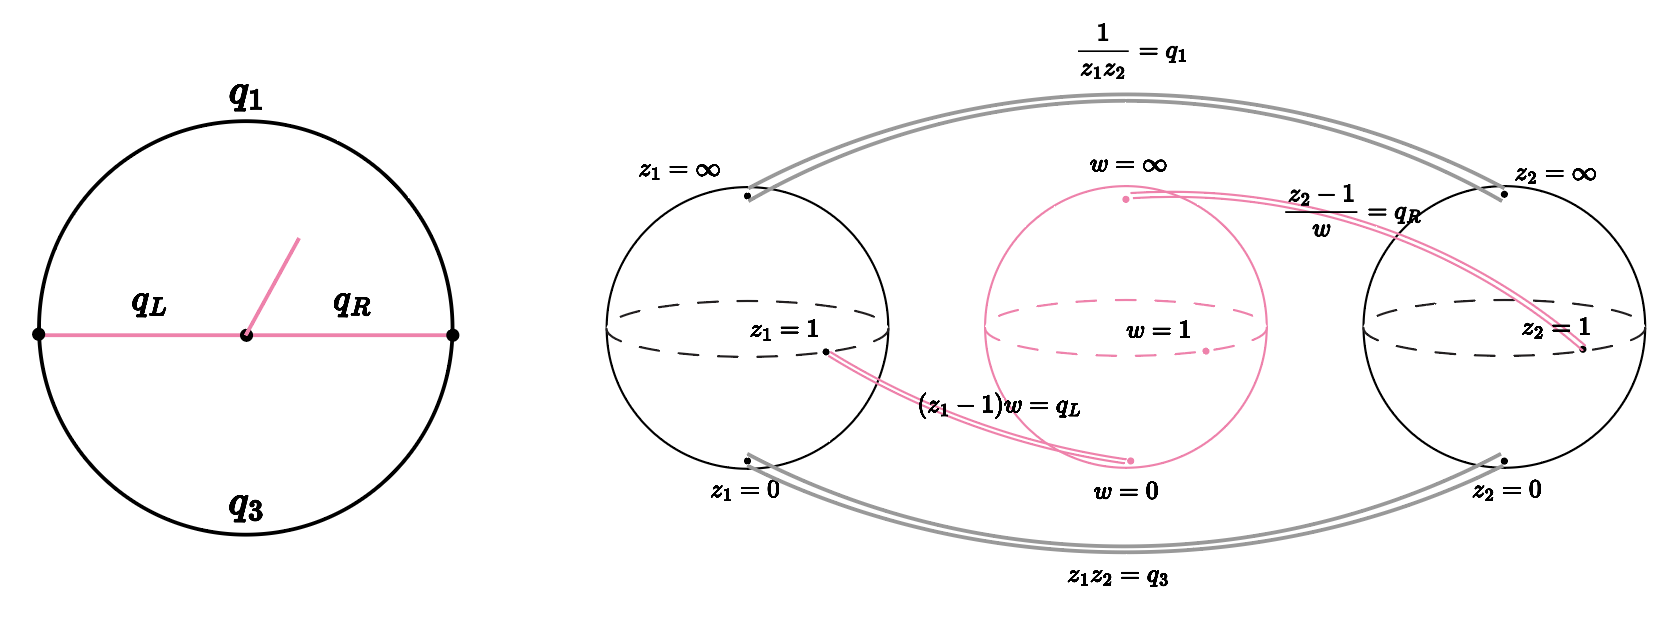
\includegraphics[scale=0.56]{figures/splitedge.png}
    \end{center}
    \caption{Splitting the second edge in the genus-2 theta channel. The second edge that connects $z_1=1, z_2=1$ in the original plumbing graph is replaced by a new sphere and two new edges shown in pink.}
    \label{fig:splitedge}
\end{figure}

We now turn to the case where the block contains odd Ramond loops. In this case, we define a new, non-vanishing enlarged block $\hat{\mathbf{F}}^{(f,\eta,a)}_f[\Theta\psi]$ by the following: For each odd Ramond loop $C$, we split one of the edges $e$ in $C$. Suppose $e$ connects two Riemann spheres with complex coordinates $z, z'$, and the punctures $e$ connects to are located at $z=z_0, z'=z_0'$. We replace $e$ by introducing a new Riemann sphere $w$, and glue the two punctures $w=0, w=\infty$ with the two original spheres $z_1, z_2$ by
\ie 
(z-z_0)w={q}_{e_L},\quad (z'-z'_0)w^{-1}=q_{e_R}.
\fe
The two new edges $e_L, e_R$ formed are both Ramond. We repeat this splitting procedure for each odd Ramond loop in $\hat{\Gamma}$, and we denote the set of all split edges by $E_\mathrm{split}$. This procedure defines a new plumbing channel ${\Gamma}_{\mathrm{split}}$, whose plumbing parameters are given by $\{q_e\}_{e\notin E_\mathrm{split}}$ and $\{q_{e_L}, q_{e_R}\}_{e\in E_\mathrm{split}}$. The original parameter $q_e$ for a split edge can be related to $q_{e_L}, q_{e_R}$ by $q_e=q_{e_L}q_{e_R}$. Similarly, the spin sign $\eta_e$ can be recovered by $\eta_e=\eta_{e_L}\eta_{e_R}$. An example of this procedure where one splitting the second edge of the genus-2 theta channel is illustrated in figure \ref{fig:splitedge}. 

On each new sphere $w$, we insert the operator $\Theta \psi$ at $w=1$, where the operator $\Theta$ acts on the fermion ground states as
\ie
\Theta u^{\mathsf{b}} = (-1)^{\mathsf{b}+1}u^{1-\mathsf{b}},
\fe
and it anticommutes with $\psi_r, G_r$ while commuting with $L_n$. The new enlarged block $\hat{\mathbf{F}}^{(f,\eta,a)}_f[\Theta\psi]$ is defined to be
\ie 
\widehat{\mathbf{F}}^{\{f,\eta,a\}}_{\hat{\Gamma}}[\Theta \psi] &= \sum_{\{A,\alpha,\mathsf{A},\mathsf{a}\}} (-1)^{K_\Gamma(\epsilon+\epsilon')} \prod_{e\in E_\NS\cup (E_\R\backslash E_\mathrm{split})} q_e^{|A_{e_1}|+|\mathsf{A}_{e_1}|}\eta_e^{\epsilon_e+\epsilon_e'}(-1)^{\epsilon_e'} \\
&\times \prod_{e\in E_\NS} \mathbf{G}_{h_e}^{A_{e_1}A_{e_2}} \prod_{e\in E_\R\backslash E_\mathrm{split}} \mathbb{G}_{\beta_e}^{A_{e_1}\alpha_{e_1},A_{e_2}\alpha_{e_2}}\\
&\times \prod_{v \in V_\NS} \hat{\rho}_{a_v}(\Psi_{-\mathsf{A}_{v_1}}\mathbf{1}\otimes \mathbf L_{-A_{v_1}}\phi_{v_1},\Psi_{-\mathsf{A}_{v_2}}\mathbf{1}\otimes \mathbf L_{-A_{v_2}}\phi_{v_2},\Psi_{-\mathsf{A}_{v_3}}\mathbf{1}\otimes \mathbf L_{-A_{v_3}}\phi_{v_3})\\
&\times\prod_{v\in V_\R}\hat{\rho}_{f_v}^{(\eta_v)}(\Psi_{-\mathsf{A}_{v_1}}\mathbf{1}\otimes \mathbf L_{-A_{v_1}}\phi_{v_1},\Psi_{-\mathsf{A}_{v_2}} u^{\mathsf{a_{v_2}}}\otimes\mathbb L_{-A_{v_2}}w_{v_2}^{\alpha_{v_2}},\Psi_{-\mathsf{A}_{v_3}} u^{\mathsf{a_{v_3}}}\otimes\mathbb L_{-A_{v_3}}w_{v_3}^{\alpha_{v_3}})\\
&\times \prod_{e\in E_\mathrm{split}} q_{e_L}^{|A_{e_1}|+|\mathsf{A}_{e_1}|}q_{e_R}^{|A_{e_2}|+|\mathsf{A}_{e_2}|}\eta_e^{\epsilon_e+\epsilon_e'}\mathbb{G}^{A_{e_1}\alpha_{e_1}, A_{e_L}\alpha_{e_L}}_{\beta_e}\mathbb{G}^{A_{e_R}\alpha_{e_R}, A_{e_2}\alpha_{e_2}}_{\beta_e}\\
&\qquad \qquad \times \langle \langle \Psi_{-\mathsf{A}_{e_2}}u^{\mathsf{a}_{e_2}}\otimes \mathbb{L}_{-A_{e_R}}w^{\alpha_{e_R}}_{e_R}|\Theta \psi(1)|\Psi_{-\mathsf{A}_{e_1}}u^{\mathsf{a}_{e_1}}\otimes \mathbb{L}_{-A_{e_L}}w^{\alpha_{e_L}}_{e_L}\rangle,
\fe
where the sum is over all displayed labels, subject to \eqref{selection} and \eqref{Fselection}, except that the fermion labels $\mathsf{A}_{e_1}$, $\mathsf{A}_{e_2}$ and $\mathsf{a}_{e_1}$, $\mathsf{a}_{e_2}$ on a split edge may differ due to the $\psi(1)$ insertion. Their combined parities are constrained to be the same, namely
\ie
(-1)^{\mathsf{A}_{e_1}+\mathsf{a}_{e_1}}=(-1)^{\mathsf{A}_{e_2}+\mathsf{a}_{e_2}},\quad e\in E_\mathrm{split}.
\fe

This enlarged block is non-vanishing, and can be expressed as a convolution of the ordinary superconformal block and the free fermion block $\mathbf{F}^{\mathsf{F}}_{\hat{\Gamma}}[\Theta \psi]$ with the same insertion $\Theta \psi(1)$ on the inserted spheres of each split edge. Namely,
\ie \label{Insconv}
\widehat{\mathbf{F}}^{\{f,\eta,a\}}_{\hat{\Gamma}}[\Theta \psi] = {\mathbf{F}}^{\{f,\eta,a\}}_{\hat{\Gamma}} \star \mathbf{F}^{\mathsf{F}}_{\hat{\Gamma}}[\Theta \psi].
\fe

On the other hand, since the operator $\psi$ can be regarded as $v_{1/2}(P)$ with Liouville momentum $P=\frac{Q}{2}$, and the operator $\Theta$ commutes with the two copies of Virasoro algebras, one can decompose $\widehat{\mathbf{F}}_f^{(\eta, \eta')}[\Theta \psi]$ into Virasoro blocks as
 \ie
\widehat{\mathbf{F}}^{\{f,\eta,a\}}_{\hat{\Gamma}}[\Theta \psi]&= \sum_{\{n,\alpha\}} (-1)^{K(\epsilon)} \prod_{e\in E_\NS} q_e^{2n_e^2}\eta_e^{2n_e} \prod_{e\in E_\R\backslash E_\mathrm{split}} q_e^{2n_e^2-\frac{1}{8}}\eta_e^{\alpha_e}\\
&\times \prod_{e\in E_\mathrm{split}} q_{e_L}^{2n_{e_L}^2-\frac{1}{8}}q_{e_R}^{2n_{e_R}^2-\frac{1}{8}} \eta_e^{\alpha_e}\ \mathbb{S}(n_{e_R}, n_{e_L}, \alpha_e)\\
&\times \prod_{i=1}^2 F_{\Gamma'}(h_{e, n_e}^{(i)},h_\psi^{(1)}, c^{(i)}) \prod_{v\in V_\NS} \mathbf{B}_{a_v}(n_{v_1},n_{v_2},n_{v_3})\\
&\times \prod_{v\in V_\R} \mathbb{B}_{f_v}^{(\eta_v)}(n_{v_1},n_{v_2},n_{v_3},\alpha_{v_2},\alpha_{v_3}),
\fe   
where $F_{\Gamma'}(h_{e}^{(i)},h_\psi^{(i)}, c^{(i)})$ stands for Virasoro conformal blocks in the new channel $\Gamma'$ with external conformal weights
\ie 
h_\psi^{(1)}=-\frac{1+2 b^2}{2\left(1-b^2\right)}, \quad h_\psi^{(2)}=\frac{b^2+2}{2\left(1-b^2\right)}
\fe
on the punctures with $\Theta \psi$ insertions. The splitting coefficient $\mathbb{S}(n_R,n_L,\alpha)$ is defined as
\ie
\mathbb{S}(n_R, n_L,\alpha) = \frac{\langle \langle v_{n_R}^\alpha|\Theta \psi(1)|v_{n_L}^{\alpha}\rangle}{\|v_{n_L}^{\alpha}\|\|v_{n_R}^{\alpha}\|}.
\fe

After knowing the coefficients $\mathbb{V}_{n,\alpha}^{1,2}, \mathbb{V}_{\pm 1,n,\alpha}^{AB}$ in \eqref{Vcoeffs}, the splitting coefficients can be solved for using the $L_1$ conformal Ward identity 
\ie
\langle\langle L_1 v_{n_R}^\alpha| \Theta \psi(1)|v_{n_L}^\alpha\rangle=\langle\langle v_{n_R}^\alpha| \Theta \psi(1)|L_{-1}v_{n_L}^\alpha\rangle,
\fe
which becomes a recursion relation for the splitting coefficients after plugging in \eqref{Vcoeffs}. After solving for the splitting coefficients and the branching coefficients, one can compute $\widehat{\mathbf{F}}^{\{f,\eta,a\}}_{\hat{\Gamma}}[\Theta \psi]$ using this decomposition, and the physical superconformal block $\mathbf{F}^{\{f,\eta,a\}}_{\hat{\Gamma}}$ can be extracted from \eqref{Insconv}. 

\section{Numerical Tests}

\label{sec:numerics}

Using the algorithm presented in Sections \ref{sec:blockdecomp} and \ref{sec:oddloop}, one can compute arbitrary superconformal blocks as a series in the plumbing parameters. We have tested our algorithm in the genus-2 theta and glasses channel, as well as the genus-3 tetrahedron channel. The plumbing graph of these channels are shown in figure \ref{fig:chanel}.

\begin{figure}
\begin{center}
        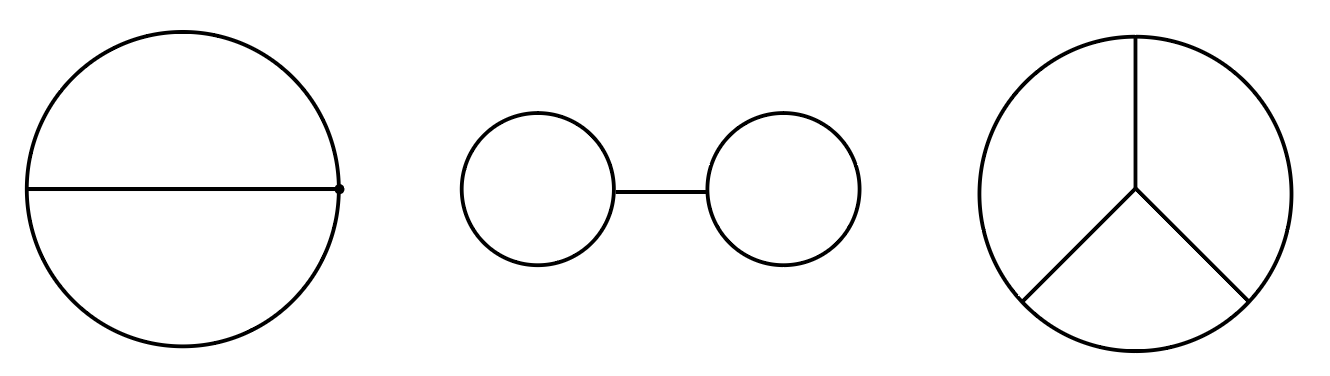
\includegraphics[scale=0.56]{figures/chanel.png}
    \end{center}
    \caption{From left to right: The genus-2 theta channel, the genus-2 glasses channel, and the genus-3 tetrahedron channel.}
    \label{fig:chanel}
\end{figure}

On a laptop and using 40-digit working precision, computing the genus-2 theta channel block with NS-R-R edges takes 7 minutes up to level $n_1, n_2, n_3\leq 10$ in the case without odd Ramond loop, and takes 27 minutes for the case with odd Ramond loop. A direct computation using the definition \eqref{scblock} is estimated to take more than 6 hours for the same block on the same device with the same precision.

For all the spin structures in the two genus-2 channels, the low-level coefficients of $q_1^{n_1}q_2^{n_2}q_3^{n_3}$ in $\mathbf{F}_\Gamma^{\{f,\eta, a\}}$ obtained from our algorithm agree with direct computations from the definition \eqref{scblock} up to level $n_1, n_2, n_3\leq 5$ for all combinations of $f_v, \eta_v, a_v$. In the theta channel and the tetrahedron channel with all NS internal edges, the superconformal block computed from our algorithm agrees with the result from $c$-recursion \cite{Belavin:2018hfm} up to level $n_1, n_2, n_3 \leq 10$. The same test has been performed for the genus-3 tetrahedron channel, where the edges around one face are Ramond while the other edges are NS. For this channel, the block $\mathbf{F}_\Gamma^{\{f,\eta, a\}}$ agrees with its definition up to total level $n_1+n_2+n_3\leq 5$, and agrees with the result of $c$-recursion up to total level $n_1+n_2+n_3\leq 10$.

Moreover, there are plumbing data $\{q_e, \eta_e\}$ in the all-NS theta channel and the NS-R-R theta channel that describe the same spin Riemann surface, and we have checked that the ratio
\ie 
\frac{Z_\text{super-Liouville}}{(Z_{\text{free boson+fermion}})^{1+2Q^2}}
\fe
of super-Liouville and free boson + fermion partition functions agrees in the two plumbing channels when evaluated using our superconformal blocks. The codes that implements our algorithm and performs the mentioned cross checks are available in a GitHub repository \footnote{Link to github}.

\section{Discussion}

\label{sec:disc}

In this work, we develop the algorithm for numerically computing superconformal blocks at arbitrary genus, in arbitrary plumbing channels, for arbitrary spin structures. The double Virasoro subalgebra allows us to decompose the enlarged $\mathsf{SCA}_\nu \oplus \mathsf{F}_\nu$ block into Virasoro conformal blocks, with the coefficients given by branching coefficients, which are known on an (NS, NS, NS) sphere and can be solved numerically using a recursion relation on an (NS, R, R) sphere.

Our algorithm provides new tools for higher-loop superstring amplitudes. For 2-dimensional Type 0B and Type 0A string theory, such amplitudes can be used to further test the duality with matrix quantum mechanics \cite{Takayanagi:2003sm,Douglas:2003up,Balthazar:2022atu,Balthazar:2022apu}, as well as the T-duality between the two theories \cite{Yin:2003iv}. They also permit direct worldsheet tests of matrix-integral predictions for recently proposed super Virasoro minimal strings \cite{Johnson:2024fkm,Johnson:2025vyz,Johnson:2026ugu,Rangamani:2025wfa,Eberhardt:2026hfh}. One particularly interesting direction is the 2-dimensional SO(23) heterotic string \cite{Davis:2005qe}, where the matrix quantum mechanical dual remains unknown, and the higher-loop or higher-point amplitudes can be used to find it. In these applications of string amplitudes, our algorithm can be used to compute the integrand on moduli space. The integration can be performed using a similar method to \cite{Christian:new}: For genus $g\leq 3$, one samples the moduli space parametrized by the period matrix and converts the period matrix into plumbing parameters using a similar algorithm to \cite{Christian:2026qqy}. 

Beyond string amplitudes, modular covariance of higher-genus partition functions can be used to constrain the spectrum and the structure constants of $\mathcal{N}=1$ SCFTs, extending the analysis of \cite{Cho:2017fzo}. The superconformal blocks themselves are conjectured to be the wavefunctions of 3D  supergravity in AdS${}_3$ \cite{Eberhardt:2026hfh}, and the numerical values of the blocks obtained from our algorithm can be used to compute gravitational path integrals in this theory \cite{Bhattacharyya:2024vnw}.

\section*{Acknowledgments}

We are grateful to Ben Mazel, Sounak Pal, Victor A. Rodriguez, and Jaroslav Scheinpflug for discussions. This work is supported by DOE grant DE-SC0007870. YW and XY thank the Yukawa Institute for Theoretical Physics for its hospitality during the course of this work. ChatGPT 5.6 Sol and 6 Astra were used in this work for drafting and editing, literature searches, algorithm implementation, and conducting numerical tests. 

\begin{appendix}

\section{Free field representation of $\mathsf{Vir}\oplus \mathsf{Vir}$ primaries}

\label{app:freefield}

The $\mathsf{Vir}\oplus \mathsf{Vir}$ primaries can be directly constructed using a free field realization of the $\mathsf{SCA}_\nu \oplus \mathsf{F}_{\nu}$ algebra \cite{Hadasz:2013dza}. Using free boson operators $\left\{c_n | n\neq 0\right\}$, free fermion operators $\left\{\eta_r| r\in \mathbb{Z}+\nu\right\}$ and the central element $\hat{P}$ that satisfy the algebraic relations
\ie
[c_n,c_m] =n\delta_{m+n,0}, ~\left\{\eta_r,\eta_s\right\}= \delta_{r+s,0},
\fe
the generators of the superconformal algebra $\mathsf{SCA}_\nu$ can be realized as
\ie
L_{n\neq 0} & =\frac{1}{2} \sum_{k \neq 0, n} c_k c_{n-k}+\frac{1}{2} \sum_r r \eta_{n-r} \eta_r+\frac{i}{2}(Q n - 2 \hat{P}) c_n, \\
L_0 & =\sum_{k>0} c_{-k} c_k+\sum_{r>0} r \eta_{-r} \eta_r+\frac{1}{2}\left(\frac{Q^2}{4}-\hat{P}^2\right)+\frac{1-2\nu}{16}, \\
G_r & =\sum_{n \neq 0} c_n \eta_{r-n}+i(Q r - \hat{P}) \eta_r.
\fe
Each free boson mode $c_n$ and free fermion mode $\eta$ can be expressed directly in terms of $G_{-r}, L_{-n}$ and $\hat{P}$. 

It can be proved that $\mathcal{M}_{\NS}(h)$ is isomorphic to the Fock space generated by acting with $c_{n<0}, \psi_{r<0}, \eta_{r<0}$ on a ground state $\phi(P)$ that satisfies $\hat{P}\phi(P)=P\phi(P)$ \footnote{We take the branch of $P$ as follows: For $h$ smaller than $Q^2/8$, $P$ is taken to be the positive root of $\frac{1}{4}Q^2-2h$. For $h$ greater than $Q^2/8$, we take $P=ip$ such that $p>0$. In the R-sector, $P$ is taken to be the positive root of $2\beta^2$ for $\beta^2 >0$ and the root with positive imaginary part for $\beta^2 <0$}, and the $\mathsf{Vir}\oplus\mathsf{Vir}$ primaries in $\mathcal{M}_{\NS}(h)$ can be constructed using the free field operators $\chi_{r}(P) = \psi_r - i\eta_r(P)$ as
\ie \label{vNS}
v_n(P) = \chi_{-\frac{4n-1}{2}}(P)\chi_{-\frac{4n-3}{2}}(P)\cdots \chi_{-\frac{1}{2}}(P)\phi(P)
\fe
where $\eta_r(P)$ is the solution of $\eta_r$ in terms of $L_n, G_r, \hat{P}$ and with $\hat{P}$ replaced by $P$. $v_n$ with negative $n$ is defined by the reflection formula
\ie
v_n(P) = v_{-n}(-P).
\fe
Similarly in the R-sector, the $\mathsf{Vir}\oplus\mathsf{Vir}$ primaries in $\mathcal{M}_{\R}(\beta)$ can be constructed by
\ie \label{vR}
v_n^{2n+\frac{1}{2}\,\text{mod}\, 2}(P) &= \chi_0(P)\chi_{-1}(P)\cdots \chi_{-(2n-\frac{1}{2})}(P)(u^0\otimes w_\beta^+),\\
v_n^{2n-\frac{1}{2}\,\text{mod}\,2}(P) &= \chi_0(P)\chi_{-1}(P)\cdots \chi_{-(2n-\frac{1}{2})}(P)\chi_0(-P)(u^0\otimes w_\beta^+),
\fe
for $n>0$, and by the reflection formula
\ie
(v^\alpha_{n}(P))_+ = (v_{-n}^\alpha(-P))_+,\quad (v^\alpha_{n}(P))_- = -(v_{-n}^\alpha(-P))_-,
\fe
for $n<0$. The subscripts $\pm$ denote the components ending in \(w_\beta^+\) and \(w_\beta^-\), respectively. 

The norms of these $\mathsf{Vir}\oplus \mathsf{Vir}$ primaries are computed in \cite{Hadasz:2013dza}. Defining the function $\ell(x,m)$ to be
\ie
 \ell(x,m)=2^{(1-(-1)^m)/16}
 \prod_{\substack{r,s\ge0,\ r+s<m\\r+s\equiv m\ (\mathrm{mod}\,2)}}
 (x+rb+s/b),\qquad m\ge0,
\fe
and $\ell(x,0)=1$. For $m<0$, we define their $\ell(x,m)$ using the reflection formula
\ie
 \ell(x,-m)=
 \begin{cases}
 \ell(Q-x,m),&m>0\text{ odd},\\
 (-1)^{m/2}\ell(Q-x,m),&m>0\text{ even}.
 \end{cases}
\fe
The BPZ norms of the $\mathsf{Vir}\oplus \mathsf{Vir}$ primaries with $n>0$ are given by
\ie
\|v_n(P)\|^2 &= (-1)^{2n} 2^{2n} \frac{\ell(2P,4n)}{\ell(Q+2P, 4n)},\\
\|v_n^0\|^2&=2^{2\lfloor M/2\rfloor+1}
               \frac{\ell(2P,4n)}{\ell(Q+2P,4n)},\\
 \|v_n^1\|^2&=-2^{2\lceil M/2\rceil}
               \frac{\ell(2P,4n)}{\ell(Q+2P,4n)},
\fe
For the norms of the $\mathsf{Vir}\oplus \mathsf{Vir}$ primaries with $n<0$, one needs to first translate them to those with $n>0$ using the reflection formulas.

The (NS, NS, NS) branching coeffieient is also fixed in \cite{Hadasz:2013dza} using the free field representation. In our convention, their result reads
\ie
\mathbf{B}_a&(n_1, n_2, n_3) = \frac{(-1)^{2n_3}(-i)^a}{\prod_{i=1}^3\sqrt{\ell(2P_i, 4n_i)\ell(Q+2P_i, 4n_i)}}\\
&\quad \times \ell\left(\tfrac{Q}{2}+P_1+P_2+P_3, 2(n_1+n_2+n_3)\right)\ell\left(\tfrac{Q}{2}-P_1+P_2+P_3, 2(-n_1+n_2+n_3)\right)\\
&\quad \times \ell\left(\tfrac{Q}{2}+P_1+P_2-P_3, 2(n_1+n_2-n_3)\right) \ell\left(\tfrac{Q}{2}-P_1+P_2-P_3, 2(-n_1+n_2-n_3)\right).
\fe
In the code, we used this formula directly for the (NS, NS, NS) branching coeffieient, while the (NS, R, R) ones are obtained from the $L_1$ Ward identities.

\section{Superconformal Ward Identities}

In this section, we summarize the choices of convention used in this paper for superconformal Ward identities. The $\mathcal{N}=1$ superconformal algebra is given by
\ie
\left[L_m,L_n\right]
&=(m-n)L_{m+n}
+\frac{c}{12}\left(m^3-m\right)\delta_{m+n,0},\\
\left[L_m,G_r\right]
&=\left(\frac{m}{2}-r\right)G_{m+r},\\
\left\{G_r,G_s\right\}
&=2L_{r+s}
+\frac{c}{3}\left(r^2-\frac14\right)\delta_{r+s,0}.
\fe

The $L_n$ Ward identity is given by
\ie
&\sum_{j\ge0}(-1)^j\binom nj\rho(L_{j-m-n+1}x_1,x_2,x_3)\\
&\quad=\sum_{j\ge0}\binom mj\rho(x_1,L_{n+j-1}x_2,x_3)
   +(-1)^n\sum_{j\ge0}(-1)^j\binom nj\rho(x_1,x_2,L_{m+j-1}x_3).
\fe
with $\rho$ being either $\rho_a$ or $\rho_f^{(\eta)}$. The $G_r$ and $\psi_r$ Ward identity requires one to choose a branch for the square root $\sqrt{z(z-1)}$, which we choose to be the following
\ie
\sqrt{z(z-1)}=
 \begin{cases}
 z\sqrt{1-z^{-1}},&z\sim\infty,\\
 \sqrt{z-1}\sqrt{1+(z-1)},&z\sim1,\\
 i\sqrt z\sqrt{1-z},&z\sim0.
 \end{cases}
\fe
With this choise of branch, the $G_r$ and $\psi_r$ Ward identities are given by
\ie
&\sum_{j\ge0}(-1)^j\binom nj
       \rho_a(G_{j-m-n+\frac12}x_1,x_2,x_3)\\
 &=\sum_{j\ge0}\binom mj\rho_a(x_1,G_{n+j-\frac12}x_2,x_3)
   +(-1)^{\epsilon_2+n}\sum_{j\ge0}(-1)^j\binom nj
                      \rho_a(x_1,x_2,G_{m+j-\frac12}x_3),
\fe \ie
 &\sum_{j\ge0}(-1)^j\binom nj
       \rho_{\mathsf{F}}(\psi_{j-m-n-\frac12}x_1,x_2,x_3)\\
 &=-\sum_{j\ge0}\binom mj\rho_{\mathsf{F}}(x_1,\psi_{n+j+\frac12}x_2,x_3)
   -(-1)^{\epsilon'_2+n}\sum_{j\ge0}(-1)^j\binom nj
                      \rho_{\mathsf{F}}(x_1,x_2,\psi_{m+j+\frac12}x_3),
\fe \ie
&\sum_{j\ge0}(-1)^j\binom{n+\frac12}{j}
 \rho_f^{(\eta)}(G_{j-m-n-\frac12}x_1,x_2,x_3)\\
 &=\sum_{j\ge0}\binom{m+\frac12}{j}
 \rho_f^{(\eta)}(x_1,G_{n+j}x_2,x_3)
 +i(-1)^{\epsilon_2+n}\sum_{j\ge0}(-1)^j\binom{n+\frac12}{j}
 \rho_f^{(\eta)}(x_1,x_2,G_{m+j}x_3),
\fe \ie
 &\sum_{j\ge0}(-1)^j\binom{n-\frac12}{j}
 \rho_{\mathsf{F}}(\psi_{j-m-n+\frac12}x_1,x_2,x_3)\\
 &=-\sum_{j\ge0}\binom{m-\frac12}{j}
 \rho_{\mathsf{F}}(x_1,\psi_{n+j}x_2,x_3)
 +i(-1)^{\epsilon'_2+n}\sum_{j\ge0}(-1)^j\binom{n-\frac12}{j}
 \rho_{\mathsf{F}}(x_1,x_2,\psi_{m+j}x_3).
\fe

\end{appendix}

\printbibliography
\end{document}
